\documentclass[crop]{standalone}

\usepackage{mhocolorpalettesthlmnord}
%\usepackage{mhotikz}
\usepackage{tikz}
\usetikzlibrary{
%arrows.meta,
backgrounds,
%fit,
%chains,
%calc,
%decorations.pathmorphing,
decorations.pathreplacing,
%decorations.text,
%matrix,
%mindmap,
%positioning,
%shapes,
%shadows
}
%\usepackage{mhomacros}
\usepackage{mhofonts}

\begin{document}

\begin{tikzpicture}[scale=1, auto]
    % Draw x^2 term as Blue Square
    \draw[fill = Blue!40, draw = Blue] (0, 0) rectangle (2, 2);
    \node[color = Blue](t1) at (1, 1) { \( x^2 \) };
    \draw[decorate, decoration = {brace, amplitude = 5pt, raise = 0.5pt, mirror}, draw = Blue, thick] (0, 0) -- (2, 0) node [ pos = 0.5, below = 5pt, color = Blue] { \( x \) };
    \draw[decorate, decoration = {brace, amplitude = 5pt, raise = 0.5pt}, draw = Blue, thick] (0 , 0) -- (0, 2) node[ pos = 0.5, left = 5pt, color = Blue] { \( x \) };
    %Draw x term as rectangle
    \draw[fill = Teal!40,draw = Teal] (2, 0) rectangle (3, 2);
    \draw[decorate, decoration = {brace, amplitude = 5pt, raise = 0.5pt, mirror}, draw = Teal, thick] (2, 0) -- (3, 0) node[ pos = 0.5, below = 5pt, color = Teal] { \( p \) };
    \draw[dashed, draw = SteelI] (2.5, 0) -- (2.5, 2);
    \node[color = Teal] (t2) at (2.5, 1) { \( px \) };
\end{tikzpicture}

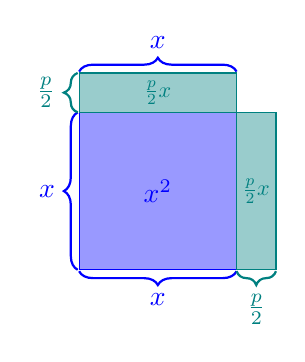
\begin{tikzpicture}[scale=1, auto]
    % Draw x^2 term as Blue Square
    \draw[fill = Blue!40, draw = Blue] (0, 0) rectangle (2, 2);
    \node[color = Blue] (t1) at (1, 1) { \( x^2 \) };
    \draw[decorate, decoration = {brace, amplitude = 5pt, raise = 0.5pt, mirror}, draw = Blue, thick] (0, 0) -- (2, 0) node [pos = 0.5, below = 5pt, color = Blue] { \( x \) };
    \draw[decorate, decoration = {brace, amplitude=5pt, raise = 0.5pt}, draw = Blue, thick] (0, 0) -- (0, 2) node [pos = 0.5, left = 5pt, color = Blue]{ \( x \) };
    % Draw x term a as rectangle
    \draw[fill = Teal!40, draw = Teal] (2, 0) rectangle (2.5, 2);
    \draw[decorate, decoration = {brace, amplitude = 5pt, raise = 0.5pt, mirror}, draw = Teal, thick] (2, 0) -- (2.5, 0) node [pos = 0.5,below = 5pt, color = Teal]{ \( \frac{p}{2} \) };
    \node[color = Teal, scale = 0.8] (t2a) at (2.25, 1) { \( \frac{p}{2}x \) };
    % Draw x term b as rectangle
    \draw[fill = Teal!40, draw = Teal] (0, 2) rectangle (2, 2.5);
    \draw[decorate, decoration = {brace, amplitude = 5pt, raise = 0.5pt}, draw = Blue, thick] (0, 2.5) -- (2, 2.5) node [pos = 0.5,above = 5pt, color = Blue]{ \( x \) };
    \draw[decorate, decoration = {brace, amplitude = 5pt, raise = 0.5pt}, draw = Teal, thick] (0, 2) -- (0, 2.5) node [pos = 0.5, left = 5pt, color = Teal]{ \( \frac{p}{2} \) };
    \node[color = Teal, scale = 0.8] (t2b) at (1, 2.25) { \( \frac{p}{2}x \) };
\end{tikzpicture}

\begin{tikzpicture}[scale=1, auto]
    % Draw x^2 term as Blue Square
    \draw[fill = Blue!40, draw = Blue] (0, 0) rectangle (2, 2);
    \node[color = Blue] (t1) at (1, 1) { \( x^2 \) };
    % Draw x term a as rectangle
    \draw[fill = Teal!40, draw = Teal] (2, 0) rectangle (2.5, 2);
    \node[color = Teal, scale = 0.8] (t2a) at (2.25, 1) { \( \frac{p}{2}x \) };
    % Draw x term b as rectangle
    \draw[fill = Teal!40, draw = Teal] (0, 2) rectangle (2, 2.5);
    \node[color = Teal, scale = 0.8] (t2b) at (1, 2.25) { \( \frac{p}{2}x \) };

    \draw[decorate, decoration = {brace, amplitude = 5pt, raise = 0.5pt}, draw = SteelI, thick] (0, 0) -- (0, 2.5) node [pos = 0.7,left = 15pt, color = SteelI, rotate = 90]{ \( x + \frac{p}{2} \) };
    \draw[decorate, decoration = {brace, amplitude = 5pt, raise = 0.5pt, mirror}, draw = SteelI, thick] (0, 0) -- (2.5, 0) node [pos = 0.5, below = 5pt, color = SteelI]{ \( x + \frac{p}{2} \) };

    % Draw k as square
    \begin{scope}[rotate = -20]
        \draw[fill = Red!40,draw = Red] (2,3) rectangle (2.5, 3.5);
        \node[color = Red, scale = 0.8, rotate = -20] (t3) at (2.25, 3.25) { \( k \) };
        \draw[decorate, decoration = {brace, amplitude = 5pt, raise = 0.5pt}, draw = Teal, thick] (2, 3.5) -- (2.5, 3.5) node [pos = 0.65, above = 5pt, color = Teal, rotate = -20]{ \( \frac{p}{2} \) };
    \end{scope}

    \begin{scope}[on background layer]
        \draw[->, draw = Red, thick] (t3) to [out = 135, in = 45](2.25, 2.25);
    \end{scope}
\end{tikzpicture}

\begin{tikzpicture}[scale=1, auto]
    % Draw x^2 term as Blue Square
    \draw[fill = Blue!40, draw = Blue] (0, 0) rectangle (2, 2);
    \node[color = Blue] (t1) at (1, 1) { \( x^2 \) };

    % Draw x term a as rectangle
    \draw[fill = Teal!40, draw = Teal] (2, 0) rectangle (2.5, 2);
    \node[color = Teal, scale = 0.8] (t2a) at (2.25, 1) { \( \frac{p}{2}x \) };
    % Draw x term b as rectangle
    \draw[fill = Teal!40, draw = Teal] (0, 2) rectangle (2, 2.5);
    \node[color = Teal, scale = 0.8] (t2b) at (1, 2.25) { \( \frac{p}{2}x \) };

    \draw[decorate, decoration = {brace, amplitude = 5pt, raise = 0.5pt}, draw = SteelI, thick] (0, 0) -- (0, 2.5) node [pos = 0.7, left = 15pt, color = SteelI, rotate = 90]{ \( x + \frac{p}{2} \) };
    \draw[decorate, decoration = {brace, amplitude = 5pt, raise = 0.5pt, mirror}, draw = SteelI, thick] (0, 0) -- (2.5, 0) node [pos = 0.5, below = 5pt, color = SteelI]{ \( x + \frac{p}{2} \) };

    % Draw k as square
    \draw[fill = Red!40, draw = Red] (2,2) rectangle (2.5, 2.5);
    \node[color = Red, scale = 0.8] (t3) at (2.25, 2.25) { \( k \) };

\end{tikzpicture}

\end{document}
